\chapter{Estado del Arte} % Estado del Arte
Antes de llevar a cabo el estudio técnico sobre la situación de las tecnologías IEEE 802.15.4, Thread y Zigbee en lo referente a las características y medidas de seguridad implementadas por cada protocolo, se introducen una serie de conceptos fundamentales sobre los que se apoyan las tecnologías analizadas en el proyecto: \textit{Domótica}, \textit{WPAN} e \textit{Internet of Things}


\section{Introducción a la domótica} % Introducción a la domótica
La domótica es el conjunto de tecnologías aplicadas al control y la automatización inteligente de las viviendas, que permite una gestión eficiente del uso de la energía aportando seguridad y confort, además de comunicación entre el usuario y el sistema. Un sistema domótico es capaz de recopilar información proveniente de diferentes sensores o entradas, procesar esa información y emitir órdenes de acuerdo a las reglas que haya establecido el usuario del sistema. La red de control del sistema domótico se integra con la red de energía eléctrica y se coordina con el resto de redes como telefonía, televisión, y tecnologías de la información.
\\Actualmente, la domótica ofrece una respuesta a los requerimientos que plantean los nuevos cambios sociales y la tendencia a incluir la tecnología en todos los aspectos de la vida humana, facilitando el diseño de edificios y hogares más personales, polifuncionales y flexibles.
\\\\
En resumen, el conjunto de tecnologías que forman el concepto de domótica, contribuyen a aumentar la calidad de vida haciendo más versátil la distribución de los hogares, pudiendo cambiar las condiciones ambientales de acuerdo a diferentes escenas predefinidas y consiguiendo que la vivienda sea más funcional al desarrollar facetas domésticas, profesionales y de ocio en un mismo hogar.
\clearpage




\section{Redes inalámbricas de área personal (WPAN)} % Redes inalámbricas de área personal (WPAN)
Las redes inalámbricas de área personal o WPAN (Wireless Personal Area Network) son redes que permiten establecer comunicaciones inalámbricas entre distintos dispositivos como computadoras, tablets, impresoras, PDAs ... los cuales se utilizan dentro del espacio de trabajo de una persona. La finalidad de este tipo de redes es comunicar cualquier dispositivo personal con sus periféricos, así como permitir una comunicación directa dentro de un área reducida entre estos dispositivos.
\\\\
En una WPAN se utilizan tecnologías de redes inalámbricas de baja potencia como Thread y Zigbee, los cuales operan en la banda de radio ISM, utilizando como base el estándar IEEE 802.15.4 producido por el IEEE 802.15, un grupo de trabajo del comité de estándares IEEE 802 del Instituto de Ingenieros Eléctricos y Electrónicos, el cual especifica los estándares de la redes inalámbricas de área personal (WPANs).
\\\\
El grupo de trabajo IEEE 802.15 ha definido tres clases de WPANs según las características de rango de datos, consumo de energía y calidad de servicio (QoS):
\begin{itemize}
\item{\bf WPANs con un rango de velocidad alto (802.15.3/ High Rate WPAN)}: diseñadas para aplicaciones multimedia que requieren altos niveles de QoS.
\item{\bf WPANs de rango medio (802.15.1/ Bluetooth)}: administran una gran cantidad de tareas (comunicaciones entre tablets, smartphones, ...) y tienen una QoS apropiada para aplicaciones de voz.
\item{\bf LR-WPANs (802.15.4/ Thread y Zigbee)}: son redes inalámbricas personales con bajas tasas de transmisión de datos entre los dispositivos que la forman. El IEEE 802.15.4 es el estándar que define el nivel físico y de control de acceso al medio en este tipo de redes.
\end{itemize}
\begin{figure}[H]
\centerline{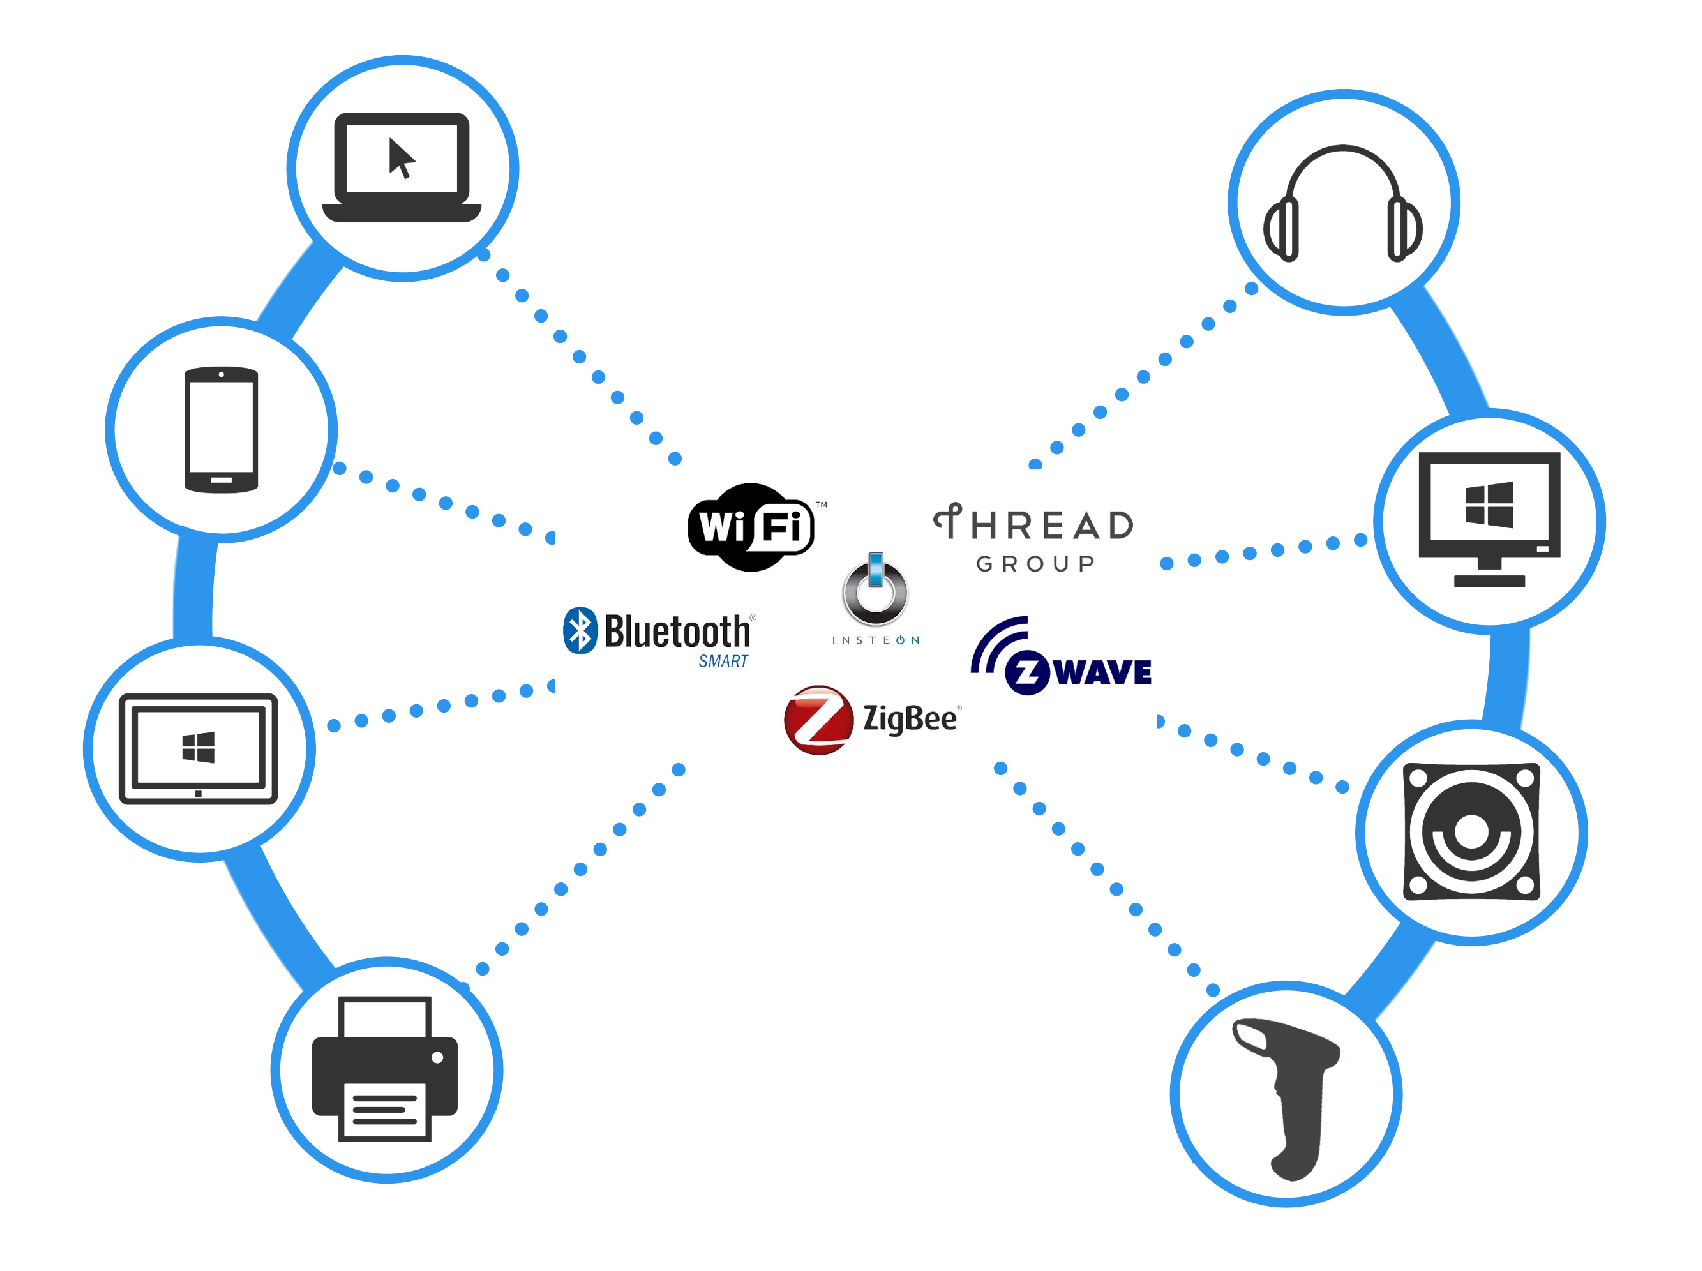
\includegraphics[width=9cm]{figuras/wpan.eps}}
\caption{Red inalámbrica de área personal (WPAN)\cite{wpan}}
\label{wpan}
\end{figure}
\clearpage




\section{El Internet de las Cosas} % Internet de las cosas
\subsection{Descripción} % Descripción
No existe una definición universal para el término IoT ( Internet Of Things / Internet de las Cosas), aunque normalmente se refiere a escenarios donde la conectividad de red y la capacidad informática se extiende a objetos, sensores y elementos cotidianos que no se consideran especificamente computadoras, lo que permite que estos dispositivos generen, intercambien y consuman datos con una mínima intervención humana. 
El término Internet of Things fue propuesto por el británico y pionero de la tecnología Kevin Ashton en 1999, para describir un sistema en el que el mundo físico está conectado a Internet mediante sensores.
\\\\El IoT es un tema emergente y plantea desafíos significativos que podrían interponerse en el desarrollo de su potencial. Las áreas clave, con las cuales están lidiando los desarrolladores de dispositivos IoT y los organismos encargados de crear estándares para la interconexión de estos dispositivos, son las siguientes:
\begin{itemize}
\item{\bf Seguridad: }los atributos de muchas implementaciones de IoT presentan \\ desafíos de seguridad únicos,  los cuales hay que abordar para garantizar la seguridad en los diferentes productos y servicios. Es una prioridad fundamental que los dispositivos IoT estén protegidos ante vulnerabilidades, especialmente a medida que esta tecnología se integra en nuestra vida cotidiana, ya que si los dispositivos están mal protegidos pueden servir como puntos de entrada potenciales para ataques cibernéticos.
\item{\bf Privacidad: }los flujos de datos y la especificación de los usuarios que ofrecen los dispositivos IoT pueden tener mucho valor para los usuarios, pero las preocupaciones sobre la privacidad y los posibles daños podrían dificultar la adopción completa de esta tecnología. Además, los dispositivos IoT están redefiniendo el debate sobre cuestiones de privacidad, ya que muchas implementaciones pueden cambiar de forma drástica cómo se recopilan, analizan, utilizan y protegen los datos personales.
\item{\bf Interoperabilidad/Normas: }aunque la interoperabilidad completa entre productos y servicios no siempre es factible, es un área clave a tener en cuenta ya que un entorno fragmentado de implementaciones técnicas de IoT puede inhibir el valor para los usuarios y la industria. Se deben utilizar estándares genéricos, abiertos y ampliamente disponibles para aportar beneficios a los usuarios.\clearpage
\item{\bf Legalidad, Reglamentos y Derechos: }el uso de dispositivos IoT plantea nuevas cuestiones legales y reglamentarias, así como amplifica los problemas legales existentes en Internet. Los datos recopilados por los dispositivos IoT son susceptibles al uso indebido, lo que puede suponer un problema legal para las empresas desarrolladoras.
\item{\bf Economía emergente y problemas de desarrollo: } el IoT ofrece beneficios sociales y económicos, lo que lo convierte en una herramienta muy prometedora para alcanzar objetivos de desarrollo sostenible.
\end{itemize}
\vspace{0.3cm}
\subsection{Características de IoT} % Características IoT
A pesar de los distintos desafíos a los que se enfrenta, el crecimiento y desarrollo del IoT está aumentando de forma notable, así como los estándares de comunicaciones inalámbricas para los dispositivos. Este auge se asocia y explica atendiendo a las siguientes características:
\begin{itemize}
\item{\bf IPv6:} la adopción del protocolo de internet versión 6 posibilita un mayor número de direcciones disponibles y por tanto de dispositivos conectados.
\item{\bf Abaratamiento y reducción del tamaño de los componentes:} hay un abaratamiento de los componentes necesarios para construir dispositivos IoT, así como una disminución de su tamaño a consecuencia de la ley de Moore.
\item{\bf Conectividad ubicua:} debido al menor coste y tamaño de los componentes y dispositivos, se consigue una capacidad de conectividad de bajo coste y alta velocidad a través de tecnologías inalámbricas. 
\item{\bf Progreso en análisis de datos:} hay un avance significativo en el análisis de datos gracias a la creación de nuevos algoritmos, el rápido avance en la potencia de cómputo, la capacidad de almacenamiento, etc.
\item{\bf Computación en la nube:} el aumento de la capacidad y disponibilidad de la computación en la nube permite que dispositivos pequeños y distribuidos interactúen con potentes capacidades de control y de análisis de back-end.
\end{itemize}
\clearpage
\subsection{Modelos de comunicaciones en IoT} % Modelos de comunicaciones del Internet de las Cosas
Los dispositivos IoT se conectan y comunican de múltiples formas. Analizar cada una de las estructuras de conexión es fundamental para comprender posteriormente los protocolos de comunicación inalámbrica entre dispositivos IoT.
\subsubsection{Comunicación de dispositivo a dispositivo} 
El modelo de comunicación de dispositivo a dispositivo representa dos o más dispositivos que se conectan y se comunican directamente entre sí, en lugar de a través de un servidor de aplicaciones intermediario. Estos dispositivos se comunican a través de muchos tipos de redes y utilizan protocolos como Zigbee, Bluetooth, Thread o Z-Wave, para establecer comunicaciones directas. Este modelo de comunicación se utiliza normalmente en sistemas domóticos, en los cuales se utilizan paquetes de datos pequeños para la comunicación entre dispositivos.
\begin{figure}[H]
\centerline{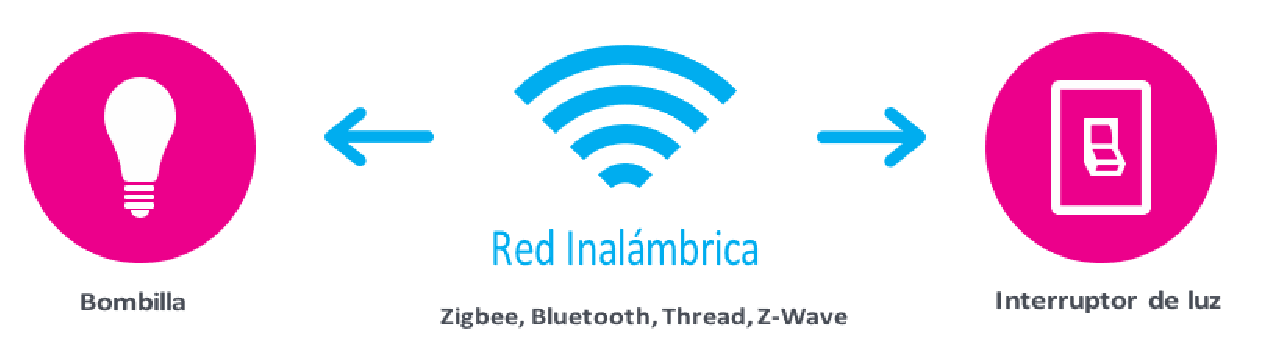
\includegraphics[width=10cm]{figuras/device-to-device.eps}}
\caption{Modelo dispositivo a dispositivo \cite{iot}}
\label{dispositivoadispositivo}
\end{figure}
\subsubsection{Comunicación de dispositivo a nube} 
En este modelo de comunicación  el dispositivo IoT se conecta directamente a un servicio en la nube en Internet. Normalmente este modelo aprovecha los mecanismos de comunicación existentes como Ethernet  o Wi-Fi, para establecer una conexión entre el dispositivo y la red IP, que en última instancia se conecta al servicio en la nube.
\begin{figure}[H]
\centerline{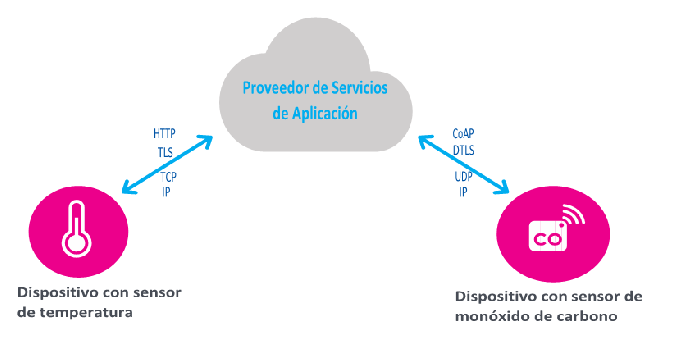
\includegraphics[width=10cm]{figuras/device-to-cloud.eps}}
\caption{Modelo dispositivo a nube \cite{iot}}
\label{dispositivo a nube}
\end{figure}
\clearpage
\subsubsection{Comunicación de dispositivo a puerta de enlace} 
También llamado modelo de dispositivo a puerta de enlace de capa de aplicación (ALG), el dispositivo se conecta a la nube a través de un servicio de ALG. Es decir, hay un software de aplicación que funciona en un dispositivo de puerta de enlace local, que actúa como intermediario entre el dispositivo y el servicio en la nube. El software se encarga de funciones como la seguridad o la traducción del protocolo.
\begin{figure}[H]
\centerline{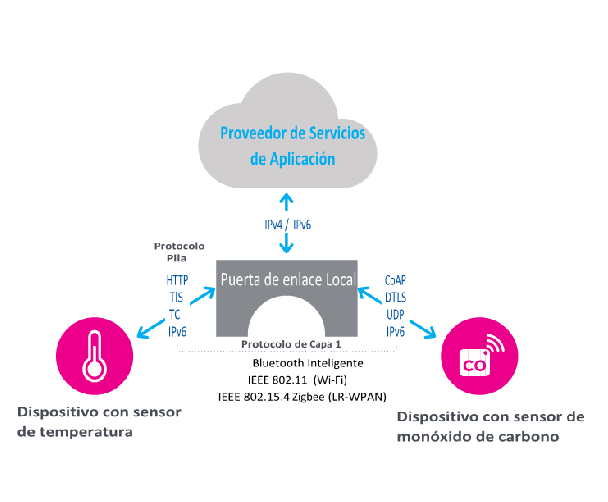
\includegraphics[width=9cm]{figuras/device-to-gateway.eps}}
\caption{Modelo dispositivo a puerta de enlace \cite{iot}}
\label{dispositivo a puerta de enlace}
\end{figure}
\subsubsection{Modelo de intercambio de datos Back-End} 
Este modelo hace referencia a una arquitectura de comunicación que permite a los usuarios exportar y analizar datos de objetos inteligentes de un servicio en la nube en combinación con datos de otras fuentes.
\begin{figure}[H]
\centerline{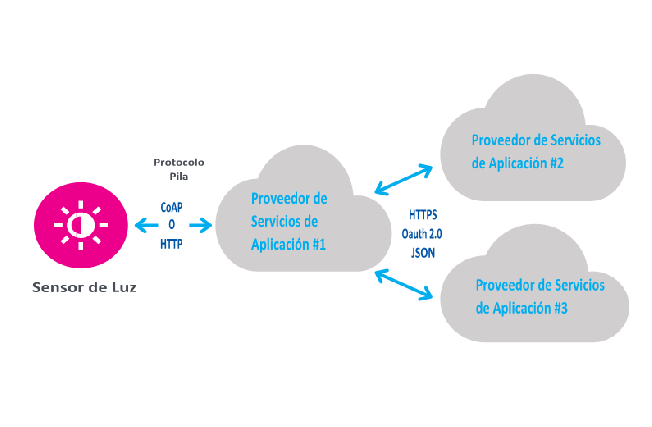
\includegraphics[width=10cm]{figuras/data-sharing-model.eps}}
\caption{Modelo de intercambio de datos Back-End \cite{iot}}
\label{intercambiobackend}
\end{figure}
\clearpage



\section{Protocolos de IoT} % Protocolos de IoT
El auge de la domótica y el IoT, ha hecho que se consoliden algunos estándares de comunicación. Entre las principales tecnologías utilizadas destacan las siguientes:
\\\\$\blacksquare$ {\underline{\textbf{Wifi}}} % Wifi
\\\\Es una tecnología consolidada que permite la interconexión inalámbrica de dispositivos electrónicos. Wifi está desempeñando un papel importante en la mayoría de entornos IoT y ya ha sido estandarizado para varios perfiles clave de IoT debido a su omnipresencia dentro de las LAN, aunque consume demasiada energía.
\\\\$\blacksquare$ {\underline{\textbf{BLE (Bluetooth)}}} % BLE
\\\\Es una tecnología de comunicación de corto alcance, bajo ancho de banda y baja latencia, muy importante en el desarrollo de aplicaciones IoT debido a sus características técnicas. BLE no ha sido diseñado para transferencia de archivos sino que es más adecuado para la transmisión de pequeños fragmentos de datos. 
\\\\$\blacksquare$ {\underline{\textbf{Z-Wave}}} % Z-Wave
\\\\Es una tecnología de comunicación de RF de baja potencia diseñada para la comunicación punto a punto y para el envío de pequeños paquetes de datos a velocidades relativamente bajas. Siendo adecuada para el envío de mensajes en aplicaciones IoT.
\\\\$\blacksquare$ {\underline{\textbf{Sigfox}}} % Sigfox
\\\\Es una tecnología de baja potencia que destaca por su amplio rango (3-10 km en entornos urbanos). Sigfox utiliza Ultra Narrow Band (UNB), que permite exclusivamente el manejo de bajas velocidades de transferencia de datos.
\\\\$\blacksquare$ {\underline{\textbf{Cellular}}} % Cellular
\\\\Es una tecnología de IoT ideal para aplicaciones que necesiten alta transferencia de datos y cuya implementación en aplicaciones de IoT requiera de operaciones de transferencia entre distancia largas. Cellular puede aprovechar las capacidades de las comunicaciones móviles GSM, 3G y 4G para proporcionar una conexiónn segura y de alta velocidad a internet. Sin embargo, necesita un alto consumo de energía.
\\\\$\blacksquare$ {\underline{\textbf{NFC}}} % NFC
\\\\Es una tecnología de comunicación inalámbrica de muy corto alcance que permite la transmisión de datos entre dispositivos, al juntarlos no más de unos pocos centímetros. NFC permite interacciones bidireccionales simples y seguras entre dispositivos, permitiendo conectar smartphones, realizar transacciones de pago, etc.
\clearpage




\section{Estándar IEEE 802.15.4} % Estándar IEEE 802.15.4
\subsection{Descripción} % Descripción
IEEE 802.15.4 es un estándar que expecifica la capa física (PHY) y la capa de control de acceso al medio (MAC) de las redes inalámbricas de área personal de baja velocidad (LR-WPAN). Este estándar define los niveles de red básicos para las LR-WPANs, centradas en la conectividad de dispositivos ubicuos de bajo coste, baja velocidad de transmisión de datos y poco consumo de energía.
\\\\
El IEEE 802.15.4 opera en la capa 2 del modelo OSI, la capa de enlace de datos, y no define los niveles superiores ni las subcapas de interoperabilidad. Sin embargo, existen protocolos como Thread y Zigbee que utilizan este estándar como base para completar la pila de comunicaciones y proponer así una solución completa.
\begin{figure}[H]
\centerline{\includegraphics[width=7cm]{figuras/ieeecapa2.eps}}
\caption{Pila del estándar IEEE 802.15.4 \cite{ieeestack}}
\label{pilaieee}
\end{figure}
\clearpage




\subsection{Tipos de dispositivos} % Tipos de dispositivos
El estándar IEEE 802.15.4 define dos tipos de nodos o dispositivos diferentes que pueden participar en una red:
\begin{itemize}
\item{\bf Dispositivo de funcionalidad completa} (FFD, Full-Function Device):
\begin{itemize}
\item Puede funcionar como un nodo central ''coordinador'', el cual gestione una red de área personal (PAN), o como un nodo normal de la red.
\item Puede establecer una comunicación con cualquier otro dispositivo.
\item Puede encaminar los mensajes de la red, denominándose coordinador PAN si es el responsable de toda la red y no sólo de su entorno.
\end{itemize}
\item{\bf Dispositivo de funcionalidad reducida} (RFD, Reduced-Function Device):
\begin{itemize}
\item Estos dispositivos no pueden ser coordinadores de la red y sólo pueden comunicarse con FFDs.
\item Son dispositivos diseñados para aplicaciones simples, que tienen comunicaciones limitadas y no utilizan muchos recursos.
\end{itemize}
\end{itemize}

\subsection{Topologías de la red} % Topologías de la red
Las redes IEEE 802.15.4 están formadas por un grupo de dispositivos que se encuentran dentro de un rango reducido, identificados dentro de la red mediante su dirección MAC (dirección de 64 bits), aunque si se dan ciertas condiciones se pueden utilizar identificadores más cortos de 16 bits. Las redes necesitan al menos de un FFD que actúe como coordinador, encargado de la creación y control de las mismas.
\\\\Dependiendo de los requisitos de la aplicación, la red puede adaptarse a una de las siguientes topologías:
\begin{itemize}
\item{\bf Topología en estrella:} se establece la comunicación entre los dispositivos de la red y un único coordinador central, el coordinador PAN. El coordinador generalmente se encuentra conectado a la corriente, y el resto de dispositivos estarán alimentados por baterías. Un ejemplo de aplicaciones que se benefician de esta topología son los sistemas de automatización del hogar, los sistemas de monitorización sanitaria o los dispositivos periféricos de un ordenador.
\begin{figure}[H]
\centerline{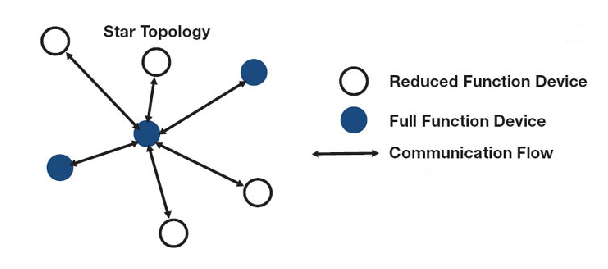
\includegraphics[width=8.6cm]{figuras/ieeestartopology.eps}}
\caption{Topología en estrella \cite{ieeetopologie}}
\label{ieeetopologiaestrella}
\end{figure}
\clearpage
\item{\bf Topología punto a punto:} en esta topología también existe un coordinador PAN, pero cualquier dispositivo es capaz de comunicarse con cualquier otro, siempre y cuando se encuentre en su rango de alcance, permitiendo formar patrones arbitrarios de conexionado y redes más complejas, como las redes en malla. El estándar no define un nivel de red por lo que no se soportan funciones de enrutamiento de forma directa. No obstante, mediante el uso de las capas superiores se permite encaminar mensajes entre dispositivos en múltiples saltos.
\begin{figure}[H]
\centerline{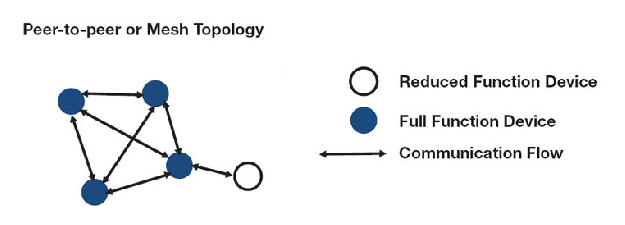
\includegraphics[width=10cm]{figuras/ieeepeertopeertopology.eps}}
\caption{Topología punto a punto \cite{ieeetopologie}}
\label{ieeetopologiamalla}
\end{figure}
\end{itemize}



\subsection{Características técnicas} % Características del estándar
El estándar IEEE 802.15.4 es la base sobre la que implementar otros protocolos de niveles superiores y es el más utilizado en comunicaciones inalámbricas para la creación de redes en IoT. Esto en parte se debe a sus características técnicas:
\\\\$\blacksquare$ {\underline{\textbf{Protección frente a ruidos y bajo consumo}}}
\\\\El estándar IEEE 802.15.4 implementa mecanismos de selección dinámica del canal para impedir fallos relacionados con la existencia de múltiples redes en una misma frecuencia, ya que diferentes protocolos como Wifi, Thread y Zigbee operan en la banda de frecuencia de 2.4GHz. Además, se limita la cantidad de energía a transmitir, permitiendo implementaciones de bajo coste y consumo.
\\\\$\blacksquare$ {\underline{\textbf{Estructura de la trama}}}
\\\\La estructura de la trama (unidad básica de transporte) ha sido diseñada para mantener la complejidad al mínimo buscando la robustez para las transmisiones en canales ruidosos.
\begin{figure}[H]
\centerline{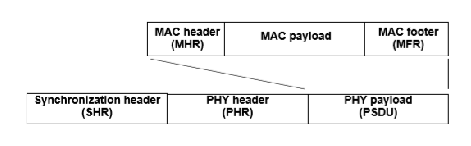
\includegraphics[width=10cm]{figuras/esquemappdu.eps}}
\caption{Esquema de la unidad de datos del protocolo (PPDU) \cite{especificacionieee}}
\label{esquemappdu}
\end{figure}
\clearpage
$\blacksquare$ {\underline{\textbf{Método de acceso}}}
\\\\La capa MAC define dos métodos para que un dispositivo acceda a la red. Estos métodos utilizan el algoritmo CSMA/CA (Carrier Sense Multiple Access-Collision Avoidance), en el cual los nodos de la red escuchan el medio antes de transmitir. Si el número de transmisiones en un determinado momento es mayor de un número especificado, el nodo espera un tiempo aleatorio e intenta la transmisión de nuevo. Existen dos tipos de implementaciones del algoritmo CSMA/CA:
\begin{itemize}
\item{\bf CSMA/CA ranurado:} este método utiliza la estructura de la supertrama (Fig. \ref{estructuratrama}), que es transmitida por el coordinador periódicamente al resto de dispositivos. Esta estructura consiste en 16 ranuras temporales (slots) de igual duración, donde la primera y última están ocupadas por las tramas baliza, que sirven para la correcta sincronización del estado (despierto/dormido) de los nodos y para informar a un dispositivo de la red que tiene una transmisión de datos pendiente. La parte activa de la supertrama es llamada el periodo de acceso de contención (CAP, Contention Access Period). En CSMA/CA ranurado, los dispositivos transmiten durante el CAP y completan la transmisión de la información dentro de la ventana temporal del CAP.
\\Sin embargo, algunos dispositivos necesitan un ancho de banda específico para transmitir información. Para solucionar esto, el coordinador de la red utiliza GTSs (Guarantee Time Slots).
\begin{itemize}
\item{\bf GTS:} el coordinador asigna un slot a los dispositivos durante el período de contención libre (CFP, Contention Free Period), utilizado por dispositivos que requieren transmisión de baja latencia. De esta manera cada uno de los nodos conoce cuando tiene que transmitir. El nodo debe enviar al coordinador un mensaje de petición GTS, al cual el coordinador contesta con un mensaje baliza que contiene el slot asignado y el número de ellos que puede utilizar.
\end{itemize}
\item{\bf CSMA/CA sin ranurado}: en este método el coordinador no transmite una baliza hasta que recibe una petición por parte de un dispositivo.
\end{itemize}
CSMA/CA y GTS evitan las interferencias y colisiones en el envío de información.

\begin{figure}[H]
\centerline{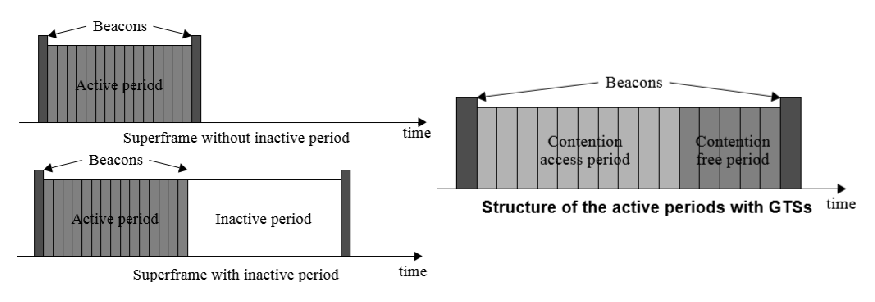
\includegraphics[width=17cm]{figuras/ieeesuperframe.eps}}
\caption{Estructura de la Supertrama \cite{especificacionieee}}
\label{estructuratrama}
\end{figure}
\clearpage




\subsection{Arquitectura} % Arquitectura
La arquitectura de IEEE 802.15.4 se define según las capas que implementa, siendo cada una de ellas responsable de una parte del estándar y de ofrecer servicios a las capas superiores.
\subsubsection{Capa Física (PHY)}
Proporciona un servicio de transmisión de datos, integrando la interfaz de gestión de la propia capa. Contiene el transceptor de radiofrecuencia (RF) junto con su mecanismo de control de bajo nivel, y permite funcionalidades como la activación y desactivación del transceptor de radio, la detección de la calidad del enlace, la selección del canal, así como la transmisión y recepción de paquetes de datos a través del medio físico.
\subsubsection{Capa de Control de Acceso al Medio (MAC)}
Proporciona acceso al canal físico de todos los tipos de transferencias, además de la gestión de la propia capa. Entre las funciones principales de esta capa se encuentran la gestión de las tramas baliza, el acceso al canal, la gestión de intervalos temporales (GTS), la validación de tramas o la asociación y disociación. Además, se encarga de habilitar la implementación de mecanismos de seguridad apropiados para las aplicaciones.
\\\\El nivel de enlace de datos hace la función de interfaz con las capas superiores de la pila de protocolos. Las capas superiores son la capa de red, que proporciona configuración y manipulación de red, y encaminamiento de mensajes, y la capa de aplicación que proporciona la funcionalidad propia del dispositivo. Estas capas se encuentran fuera del alcance de este estándar, son implementadas por los protocolos Thread y Zigbee que utilizan IEEE 802.15.4 como base.


\clearpage
\subsection{Modelos de transferencia de datos} % Modelos de transferencia de datos
El estándar IEEE 802.15.4 utiliza varios modelos de transferencia según la trayectoria de la información a transmitir.
\subsubsection{Transferencia de datos a un coordinador}
Cuando un dispositivo quiere enviar información a un coordinador en una PAN se pueden dar dos casos:
\begin{itemize}
\item{\bf La red utiliza transferencia de balizas:} el dispositivo escucha el medio hasta que encuentra una baliza, en ese momento el dispositivo se sincroniza con la estructura de la supertrama (utilizada por el coordinador para la sincronización de la PAN) y compite con el resto de dispositivos de la red utilizando CSMA/CA ranurado hasta lograr transmitir su trama de datos.
\item{\bf La red no tiene habilitada la transferencia de balizas}: el dispositivo transmite su trama de datos directamente al coordinador, utilizando CSMA/CA sin ranurado temporal.
\end{itemize}
\subsubsection{Transferencia de datos desde un coordinador}
Como en el caso anterior, este modelo de transferencia diferencia entre la posibilidad de que la red implemente o no la transferencia de balizas: 
\begin{itemize}
\item{\bf La red utiliza transferencia de balizas}: el coordinador indica con una baliza que dispone de datos para transmitir a un dispositivo. Dado que los dispositivos escuchan la red de forma periódica, este transmite una orden de petición de datos ''Data Request'' al coordinador. Finalmente, la trama de datos es enviada por el coordinador y se elimina de la lista de mensajes pendientes.
\item{\bf La red no tiene habilitada la transferencia de balizas}: en este caso, el coordinador almacena los datos para que el dispositivo apropiado los solicite. Un dispositivo solicita datos mediante la transmisión de una orden de petición de datos a su coordinador. Si una trama de datos está pendiente, el coordinador transmite la trama de datos. Sin embargo, si no existe ninguna información pendiente, el coordinador puede indicarlo de dos formas. Si se solicitó la información, se envía una trama ACK después de la orden de petición, en caso contrario se envía una trama de datos con una carga útil de longitud cero.
\end{itemize}
\subsubsection{Transferencia de datos entre pares (Peer-to-peer)}
Los dispositivos pueden tranmistir directamente cuando disponen de acceso al canal, o utilizar otra serie de medidas, las cuales están fuera del alcance del estándar, con el fin de lograr la sincronización y comunicación entre los dispositivos.


\clearpage
\subsection{Seguridad en IEEE 802.15.4} % Seguridad en IEEE 802.15.4
La seguridad en IEEE 802.15.4 está limitada por la propia naturaleza de una red inalámbrica de dispositivos de bajo coste y capacidades limitadas en términos de potencia de cálculo, de almacenamiento disponible y de consumo de energía. Estas restricciones limitan severamente la elección de los algoritmos y protocolos criptográficos a usar en las comunicaciones e influyen en el diseño de la arquitectura de seguridad. Otro factor a tener en cuenta es que las comunicaciones en redes que implementen IEEE 802.15.4 pueden implicar relaciones a corto plazo entre dispositivos, por lo tanto el establecimiento y mantenimiento de relaciones de confianza se deben de abordar con cuidado para gestionar la seguridad.
\\\\El estándar proporciona los siguientes servicios de seguridad:
\begin{itemize}
\item{\bf Confidencialidad de los datos:} se asegura que la información transmitida no sea vista por personas no autorizadas.
\item{\bf Autenticidad de los datos:} se verifica la identidad del origen y destino de la información.
\item{\bf Protección contra repetición:} garantiza que se detecta el envío de información duplicada.
\end{itemize}
La capa MAC es la encargada de proporcionar estos servicios de seguridad a las tramas salientes y entrantes, cuando se demanda por las capas superiores. No obstante, la implementación de estos servicios de seguridad es opcional y los dispositivos se comportarán de varias formas en función de esta configuración:
\begin{itemize}
\item{\bf Los dispositivos no implementan seguridad}: no se propociona un mecanismo criptográfico a la capa MAC para realizar transformaciones en las tramas salientes y entrantes.
\item{\bf Los dispositivos implementan seguridad}: se propociona un mecanismo criptográfico a la capa MAC, realizando transformaciones en las tramas salientes y entrantes.
\end{itemize}
Cuando los dipositivos implementan seguridad, se modifican varios campos de la capa MAC:
\begin{itemize}
\item{\bf Control de trama} (Frame Control) 
\item{\bf Cabecera de Seguridad Auxiliar} (Auxiliary Security Header)
\item{\bf Carga de datos útil} (Data Payload)
\end{itemize}
\clearpage
La cabecera de seguridad auxiliar (Auxiliary Security Header) solo se habilita cuando el subcampo ''Security Enabled'' está activo. Esta cabecera consta de tres campos especiales:
\begin{itemize}
\item{\bf Security Control} (1 byte), especifica la clase de protección a utilizar y la política de seguridad. Los dos primeros bits (Security Level) determinan qué se va a cifrar y la longitud de la clave. En la siguiente tabla se describen las múltiples opciones:
\begin{table}[H]
\begin{center}
\begin{tabular}{| p{3cm} | p{10cm} |} \hline
Valor & Descripción \\ \hline\hline
0x00 & Sin cifrado\\ \hline\hline
0x01 a 0x03 & Autenticación, utilizando el Código de Autenticación de Mensaje (MAC) \\ \hline\hline
0x04 & Se cifra la carga útil asegurando la confidencialidad de los datos \\ \hline\hline
0x05 a 0x07 & Se asegura la confidencialidad, la integridad y la autenticidad de los datos\\ \hline\hline
\end{tabular}
\caption{Valores del campo Security Control \cite{especificacionieee}}
\label{valoressecuritycontrol}
\end{center}
\end{table}
\item{\bf Frame Counter} (4 bytes), es un contador dado por el origen de la trama para proteger el mensaje ante ataques de repetición. Cada mensaje tendrá un ID único especificado por este campo.
\item{\bf Key Identifier} (0-9 bytes), especifica la información necesaria para conocer la clave que se está usando con el nodo destino de la comunicación.
\end{itemize}
\begin{figure}[H]
\centerline{\includegraphics[width=12cm]{figuras/ieeemacheader}}
\caption{Campos de cabecera de Seguridad Auxiliar IEEE 802.15.4 \cite{cabecerasieee}}
\label{camposseguridadauxiliar}
\end{figure}
\clearpage
En cuanto al campo de datos de carga útil puede tener tres configuraciones diferentes según los campos de seguridad definidos:
\begin{itemize}
\item{\bf AES-CTR:} todos los datos se cifran usando el algoritmo AES con una clave de 128 bits. El campo Frame Counter establece un ID único de mensaje y el  campo Key Control es usado por la capa de aplicación, si se alcanza el valor máximo de Frame Counter.
\item{\bf AES-CBC-MAC:} el Código de Autenticación de Mensaje (MAC) depende del nivel de seguridad especificado en el campo Security Policy, y se crea cifrando la información de la cabecera MAC y la carga de datos útil.
\item{\bf AES-CCM:} es un cifrado genérico que combina los dos métodos anteriores, adoptando los campos de AES-CTR y AES-CBC-MAC.
\end{itemize}
El formato adoptado por el campo de carga útil según los subcampos de seguridad definidos, sería el siguiente:
\begin{figure}[H]
\centerline{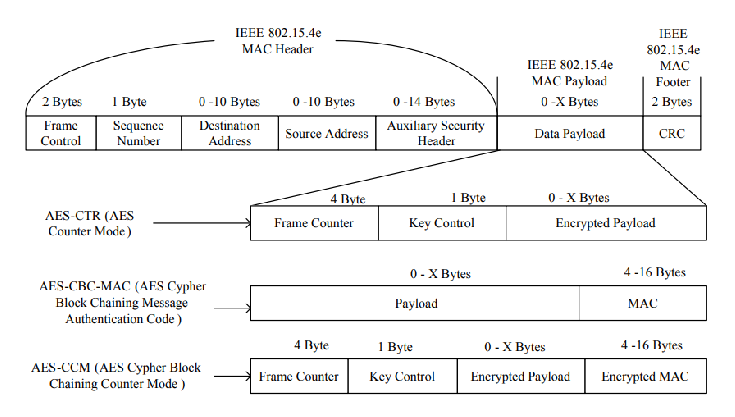
\includegraphics[width=12cm]{figuras/ieeeaes}}
\caption{Formato de carga útil correspondiente al nivel de Seguridad \cite{cabecerasieee}}
\label{formatocargautil}
\end{figure}
Los dispositivos que operan en modo seguro, tienen que controlar una lista de control de acceso (ACL, Access Control List) en la cual se almacena la dirección del nodo con el que se quiere comunicar, la política de seguridad a utilizar (AES-CTR, AES-CBC-MAC, AES-CCM), la clave, un vector de inicialización y un contador de repeticiones. De esta forma cuando un nodo quiere recibir un mensaje de otro nodo, primero se comprueba que dicho nodo se encuentra en su ACL y se transmite la información aplicando la configuración específica. En caso contrario, comienza el proceso de autenticación con el nodo.











